\section{Corpus study}
\label{sec:corpusstudies}


\subsection{Corpus choice and sampling}
\label{sec:gettingdata}

% TODO Quote:
% Brems (2016:171--175) for using GOOGLE data, including COUNTS!

For the present study, I used the German \textit{Corpus from the Web} (COW) in its 2014 version DECOW14A (\citealp{SchaeferBildhauer2012full}, and \citealp{Schaefer2015b}, as well as \citealp{BiemannEa2013}, and \citealp{SchaeferBildhauer2013}, for overviews of web corpora in general and the methodology of their construction), which contains almost 21 billion tokens.%
\footnote{The COW corpora (Dutch, English, French, German, Spanish, Swedish) are made available for free at \url{https://www.webcorpora.org}.
At the time of this writing, a newer 2016 version DECOW16 has already been released.}
I chose this corpus for two main reasons.%
\footnote{The use of web data for linguistic research does require explicit and careful justification.
Due to the noisy nature and unknown composition of the web, only carefully designed and established web corpora like the COW corpora or the SketchEngine corpora \citep{KilgarriffEa2014} should be used.
Clearly, using search engine results is ``bad science'' for many reasons, most prominently total non-replicability of results, as \cite{Kilgarriff2006} pointed out more than ten years ago.
Careless use of search engine results is still found, however, see for example \citet[171--175]{DeclerckBrems2016}.}
First, the external validity of any study is increased through a higher heterogeneity of the sample \citep[30]{MaxwellDelaney2004}, and the DECOW corpus has clearly a much more heterogeneous composition compared to the only other very large corpus of German, the DeReKo \citep{KupietzEa2010} of the Institute for the German Language (IDS), which contains almost exclusively newspaper texts.%
\footnote{It was shown in \cite{W16-2601} that, for example, the range of topics covered is much smaller in DeReKo compared to DECOW.}
Second, it was already mentioned that normative grammars often adopt clear positions regarding the grammaticality of either the \NACa\ or the \PGCa.
Thus, newspaper text or any other text that conforms strongly to normative grammars might not represent the alternation phenomenon fully (and without bias) because authors and proofreaders who must adhere to normative guidelines might favour one alternative or the other explicitly.
Web corpora, on the other hand, contain at least some amount of non-standard language from forums and similar sources.
For these or similar reasons, COW corpora have been used in a number of peer-reviewed publications, for example \cite{VanGoethemHiligsmann2014}, \cite{VanGoethemHuening2015}, \cite{MuellerS2014}, \cite{Schaefer2016c}, \cite{SchaeferSayatz2014}, \cite{SchaeferSayatz2016}, and \cite{Zimmer2015}. 
Therefore, DECOW is a valid choice for this study.

I now turn to the sampling procedure applied to obtain concordances for manual annotation and statistical analysis.
Among the factors potentially influencing the alternation (see Section~\ref{sec:germanmeasurenps}) were lemma-specific preference effects.
Therefore, it was highly desirable to obtain a sample in which most of the highly frequent actually-occurring combinations of kind nouns and measure nouns were represented.
I applied a three-stage process in order to obtain such a sample, which consisted of the following steps:

\begin{enumerate}[i.]
  \item\label{enum:data:step1} generating a list of the one hundred most frequent mass nouns,
  \item\label{enum:data:step2} deriving a list of all measure nouns with which the mass nouns co-occur in the \NACb, and 
  \item\label{enum:data:step3} sampling the target constructions by querying each combination of mass noun and measure noun found in step (\ref{enum:data:step2}).
\end{enumerate}

\vspace{-1\baselineskip}

In step (\ref{enum:data:step1}), I exported a list of all nouns in the DECOW14A01 sub-corpus sorted by their token frequency and manually went through it from the most frequent noun downwards, selecting the first one hundred mass nouns that occurred in the list.%
\footnote{DECOW14A01 is the first slice (roughly a twentieth) of the complete DECOW14A corpus.
It contains just over one billion tokens.}
Mass nouns were defined as concrete nouns which denote a substance in the broad sense, combine with uninflected mass quantifiers such as \textit{viel} `much' and \textit{wenig} `little' (\textit{viel Bier} `much beer'), and form only sortal and unit plurals (such as the plural \textit{Biere} `types of beer' or `glasses of beer').
Abstract nouns which partially behave like mass nouns (like \textit{Spaß} `fun’ or \textit{Gefahr} `danger’) were excluded because they are usually not quantified in the same way as concrete mass nouns.
The hundredth selected mass noun was \textit{Schmuck} `jewellery’, which is the 3,054th most frequent noun in the original frequency list.

This list of mass nouns was used in step (\ref{enum:data:step2}) to derive a list of measure nouns co-occurring with the mass nouns. 
In order to generate this list, I utilised the fact that a direct sequence of two nouns almost always instantiates the bare-noun NAC if the second noun is a mass noun.
Hence, I searched for all sequences N\Sub{1}N\Sub{2} where N\Sub{2} was one of the mass noun lemmas extracted in step (\ref{enum:data:step1}).
Then, the resulting 100 lists of noun-noun combinations were each sorted by frequency in descending order and sieved manually to remove erroneous hits.
From each of the 100 lists, I also removed noun-noun combinations that had a frequency below 2, except if the individual list would have otherwise been shorter than 20 noun-noun combinations.
The result was a list of the most frequent 2,365 individual combinations of a measure noun and a mass noun.

In step (\ref{enum:data:step3}), each of these 2,365 noun–noun combinations was queried in the target constructions (\PGCa\ and \NACa) individually in each of the first ten slices of DECOW (roughly 10 billion tokens).
In order to reduce the sample size for the manual annotation process, the final concordance was sampled from the results of these 2,365 queries.
Since the mass nouns in the sample were distributed according to the usual power law (often referred to as a \textit{Zipfian} distribution), I used all hits for nouns with a frequency up to 100 and a sample of 100 of all those with higher frequency.
The final sample contained 6,843 sentences, which was reduced to 5,063 in the manual annotation process due to removal of noisy material, erroneous hits and uninformative cases where the measure noun was in the genitive, in which case the \NACa\ cannot be distinguished from the \PGCa.
Given the careful sampling procedure described in this section, we can be highly sure that it contains all relevant and reasonably frequent noun–noun combinations in the target constructions.%
\footnote{In a similar fashion, the 100 most frequent measure nouns occurring with plural kind nouns were listed and queried, resulting in a sample of 871 sentences.
As stated in Section~\ref{sec:germanmeasurenps}, the \NACa\ is virtually never used with plural kind nouns, and this sample was not used except for quantifying the frequency of occurrence of the constructions (67 times \NACa\ and 794 times \PGCa).
However, the sample is distributed with the data package accompanying this paper.
}

Finally, two auxiliary samples were also drawn.
As mentioned in Section~\ref{sec:analyses}, the distribution of the measure noun and kind noun lemmas in the \NACb\ and the \PGCd\ with a determiner will be modelled as factors influencing the alternation.
Therefore, all noun-noun pairs from the process described above were also queried in the two non-alternating constructions, resulting in 17,252 hits for the \PGCd\ and 315,635 hits for the \NACb.


%%%%%%%%%%%%%%%%%%%%%%%%%%%%%%%%%%%%%%%%%%%%%%%%%%%%%%%%%%%%%%%%%%%%%%%
%%%%%%%%%%%%%%%%%%%%%%%%%%%%%%%%%%%%%%%%%%%%%%%%%%%%%%%%%%%%%%%%%%%%%%%

\subsection{Variables and annotation}
\label{sec:annotation}

The full set of manually annotated variables for the main sample is given in Table~\ref{tab:variables}, and I briefly discuss it now.%
\footnote{All numeric variables were also z-transformed (\ie\ centered to the mean and rescaled such that they have a standard deviation of 1) to facilitate their interpretation in the regression models reported in the next section.}
Notice first that \textit{Construction} is the response variable (or `dependent variable') with the values \textit{PGCa} and \textit{NACa}.

\begin{table}
  \centering
  \begin{tabular}{llll}
    Unit of reference & Variable                      & Type    & Levels (for factors only) \\
    \midrule
    Document       & Badness                          & numeric &                           \\
                   & Genitives                        & numeric &                           \\
    Sentence       & Cardinal                         & factor  & Yes, No                   \\
                   & \textbf{Construction (response)} & factor  & NACa, PGCa                \\
                   & Measurecase                      & factor  & Nom, Acc, Dat             \\
    Kind lemma     & Kindattraction                   & numeric &                           \\
                   & Kindfreq                         & numeric &                           \\
    Measure lemma  & Measureattraction                & numeric &                           \\
                   & Measureclass                     & factor  & Physical, Container,      \\
                   &                                  &         & Amount, Portion, Rest     \\
                   & Measurefreq                      & numeric &                           \\
  \end{tabular}
  \caption{Annotated variables for the main sample}
  \label{tab:variables}
\end{table}

The variables \textit{Kindattraction} and \textit{Measureattraction} encode the ratio with which a given kind noun lemma or measure noun lemma occurs in the \PGCd\ and the  \NACb.
They were calculated from the auxiliary samples described at the end of Section~\ref{sec:gettingdata} as a log-transformed quotient.
The higher the value, the more often the noun occurs in the \PGCd (proportionally).%
\footnote{
  It could be argued that some more advanced measure of attraction strength should be used, as is done in Collostructional Analysis \citep{StefanowitschGries2003,GriesStefanowitsch2004}, see also \cite{Gries2015a}.
  Three main points speak against such an approach in the present case.
  First, the goal here is to quantify how often lemmas occur in the \PGCd\ and the \NACb, and these constructions do not compete at all but are rather mutually exclusive.
  Collostructional approaches are not made for such scenarios.
  Second, the attraction values will be used as regressors in a hierarchical logistic regression and the values resulting from collostructional analysis, \ie\ logarithmised Fisher p-values, have a very unfavourable distribution in the case at hand.
  They cluster around 0 and they include values of $-\infty$.
  Third, I tried using collexeme strength as a regressor (with smoothing to remedy the mathematical problems), and the results were unsatisfactory compared to the simple quotient used here.
}
Additionally, \textit{Kindfreq} and \textit{Measurefreq} are the logarithm-transformed frequencies per 1,000,000 words of each lemma, extracted from the frequency lists distributed by the DECOW corpus creators on their web page.
They were added to control for basic frequency effects.

In Section~\ref{sec:analyses}, it was hypothesised that classes of measure lemmas might have different preferences for the two alternants.
To capture this, class information was annotated for measure lemmas.
The classification was inspired by the list in \citet[530]{Koptjevskaja2001} but due to the low frequencies of many of the potential classes, a very coarse classification was finally used.
With typical examples and their frequencies in the final sample, the classes are:
\textit{Physical} (abstract precisely measurable units such as \textit{Liter} `litre', \textit{Meter} `metre', \textit{Gramm} `gram'; \textit{f=}1,968),
\textit{Container} (\textit{Eimer} `bucket'; \textit{f=}740),
\textit{Amount} (\textit{Menge} `amount'; \textit{f=}1,364), 
\textit{Portion} (natural portions like \textit{Happen} `bite' or \textit{Krümel} `crumb'; \textit{f=}713).
The lemmas that did not fit into either of these classes were labelled \textit{Rest} (\textit{f=}278).

The variable \textit{Cardinal} encodes whether the measure noun is modified by a cardinal (\textit{f=}1,939) or not (\textit{f=}3,124).
The purpose of this variable is to test whether cardinals really favour the \NACa\ as hypothesised in Section~\ref{sec:analyses}.

To capture the influence of style mentioned in Section~\ref{sec:analyses}, two proxy variables were used.
At the document level, the DECOW corpus has an annotation for \textit{Badness}.
As described in \cite{SchaeferEa2013}, \textit{Badness} measures how well the distribution of highly frequent short words in the document matches a pre-generated language model for German.
Documents with higher Badness usually contain more incoherent language, shorter sentences, etc.
If the \PGCa\ actually favours higher stylistic levels, a high \textit{Badness} should be correlated with fewer occurrences.
Documents in DECOW14 have also been annotated with a variable called \textit{Genitives}.
The higher the values of this variable, the lower the proportion of genitives among all case-bearing forms is.
A high number of genitives is indicative of higher levels of style.
However, the use of this variable as a regressor in the present study might be considered problematic.
Since the \PGCa\ contains a genitive itself, the regressor variable \textit{Genitive} and the document-level variable \textit{Genitives} are not fully independent.
Since instances of the \PGCa\ make up for only a minute fraction of all genitives, I still use \textit{Genitives} as a regressor with the appropriate caveats.

Finally, one variable was added as nuisance variable in the context of the present study.
It was reported in the literature that MNPs in the dative and with a masculine or neuter kind noun favour the \PGCa\ more than the corresponding nominative and accusative MNPs \citep{Hentschel1993,Zimmer2015}.
As an example, \textit{mit einem Stück frischen Brots} `with a piece of fresh bread' (\PGCa) would be preferred more strongly against \textit{mit einem Stück frischem Brot} (\NACa).
As with all the examples, native speakers of German will most likely notice that differences are subtle.
To control for this effect, the case of the measure noun was manually annotated (variable \textit{Measurecase}).


%%%%%%%%%%%%%%%%%%%%%%%%%%%%%%%%%%%%%%%%%%%%%%%%%%%%%%%%%%%%%%%%%%%%%%%
%%%%%%%%%%%%%%%%%%%%%%%%%%%%%%%%%%%%%%%%%%%%%%%%%%%%%%%%%%%%%%%%%%%%%%%

\subsection{On statistical analysis}
\label{sec:rightstatistics}

In this section, I justify my choice of statistical models used in Section~\ref{sec:corpushierarchicalmodel}.
Readers might think that the method used here for modeling grammatical alternations -- namely (Hierarchical) Logistic Regression\slash Generalised Linear (Mixed) Models or GL(M)Ms -- does not require much justification.
After all, GLMMs have been established as the major tool in the analysis of alternation phenomena.
All studies mentioned at the outset of Section~\ref{sec:cogocl} use some form of regression\slash GLMM.
Over the past few years, however, modified or alternative methods have been proposed.
While it is impossible to discuss all of these methods here, I just make a few remarks on Bayesian estimation (see \citealp{GelmanEa2014}) as it was proposed in \cite{Levshina2016} and \cite{Divjak2016a}, for example.
Conceptually, I see three points of discussion that should be kept apart.
First, Bayesian methods are sometimes touted as superior tools for scientific inference compared to frequentist methods.
Second, it has been proposed that the Bayesian interpretation of probability is more cognitively adequate for the modeling of linguistic data \cite[301--302]{Divjak2016a}.
Third and very specific to this paper, given established methods in the modeling of alternation and variation, it has to be decided whether so-called Bayesian methods lead to substantially different results.

% As for the first point, this is not quite the place to discuss it fully.
% The basic distinction is a philosophical one and related to the concepts of \textit{direct} and \textit{inverse probability} (\eg\ \citealp{Senn2011}).
% Frequentists assume that models and parameters are fixed, for example a model specifying that a coin is fair.
% We can then calculate for observed data (for example a measurement of 3 heads in an experiment with 10 tosses) how often such a result or a more extreme result would occur if the model were true and we repeated the experiment arbitrarily often.
% This is essentially the frequentist notion of direct probability, \ie\ long-run frequencies under replication.
% Standard tests in the Fisher and Neyman-Pearson traditions as well as Neyman confidence intervals are based on this concept of probability.
% Bayesian approaches (in the now common interpretation), on the other hand, condition on the particular data and quantify inductively the probability of model parameters given the data.
% The parameters are thus not fixed, and the probability is usually equated with researchers' posterior beliefs about model parameters.
% There is actually a debate among Bayesians about the proper interpretation of Bayesian methods, and whether a notion of hypothesis testing is compatible (or even already contained) in the Bayesian approach.
% In \citet[10]{GelmanShalizi2013}, the authors -- prominent Bayesians themselves -- acknowledge that a theory of statistical testing is a desideratum, and they state about the standard inductive interpretation of Bayesianism that ``most of this received view of Bayesian inference is wrong,'' and they develop a Bayesian notion of p-values (see also \citealp{Mayo2013}, for a frequentist reply; also \citealp{Senn2011} on different strands of Bayesianism and their stance on inductive vs.\ deductive reasoning, and \citealp{Mayo2011}, for a critical reply to \citealp{Senn2011}).
% Clearly, in such quarrels between and among camps of philosophers of science and statisticians, it is difficult for mere practitioners to take sides.
% 
% These quarrels relate to the second point, however.
% \citet[301--302]{Divjak2016a} speaks favourably of Bayesian methods because the Bayesian concept of probability is more adequate for cognitive modeling compared to the frequentist one.
% Her argument is part of a larger body of literature asking for cognitively plausible modeling techniques, for example Naive Discriminative Learning (NDL; \citealp{Baayen2011,BaayenEa2013,MilinEa2016,TheijssenEa2013}). 
% On p.\ 303 of \cite{Divjak2016a}, the author goes on to explicitly mention NDL as well.
% Yet, neither frequentist nor Bayesian methods were conceived as cognitive models, but as systems of inference for scientists (see above, and see also \citealp[302]{Divjak2016a}).
% The fundamental question that lurks behind such arguments is how we interpret our statistical models (estimated on corpus data).
% Are they inductive models of cognitive representations that also human learners would infer from being exposed to the corpus data?%
% \footnote{In which case we are doing ``data science in language research'' in the words of \citealp{MilinEa2016}.
% I see this as standing in contradiction to the view advocated in \cite{Dabrowska2016} as cited above.}
% Or are they tests of theories that are pre-specified and merely tested for predictive accuracy on linguistic output data contained in corpora?
% In the former case, we adopt a strong \textit{corpus as input} hypothesis and should definitely resort to methods like NDL.
% However, this would most likely require us to toss most previous work done in (cognitive) linguistics into the bin and to abandon all high-level generalisations that most existing studies have been based upon.
% In fact, arguments to this extreme effect and against using high-level generalisation have been made, for example in \cite{BaayenEa2016}, \citet[299--300]{Divjak2016a}, \cite{RamscarPort2016}, \cite{TheijssenEa2013}.
% In the latter and less extreme case, the cognitive commitment does, however, not necessarily extend to the statistical methods used.
% These methods then do not need to be any more cognitively plausible than an ANOVA used to analyse the results from an experiment.
% I view my own work (see Sections~\ref{sec:germanmeasurenps}--\ref{sec:experimental}) in the tradition of testing theories (which embrace high-level generalisations), and I agree to provisionally use Likelihood methods (see below).
% I remain fully agnostic with respect to the question, which approach is \textit{right}.
% The best strategy for cognitive linguistics as a field might be to cultivate many methods while making sure that each method is applied carefully and competently.

The first and second point cannot be discussed in detail here.%
\footnote{However, there is a number of critical papers by statisticians (even prominent Bayesians) and philosophers of science in which the extreme credibility that has recently been assigned to (subjective and automatic) Bayesian approaches (and especially the standard inductivist interpretation of Bayesianism) is questioned (for example, \citealp{GelmanShalizi2013,Mayo2011,Senn2011}).}
With regard to the third point, \citet[251--252]{Levshina2016} argues for Bayesian estimation in mixed regression settings.
First, she claims that ``while frequentist statistics only allows one to test whether the null hypothesis can be rejected, Bayesian statistics enables one both to test the null hypothesis and to estimate the probability of specific parameter values given the data.''
This does not do justice to frequentist methods in that a strong focus on the rejection of the null hypothesis is characteristic only of Fisher's approach.
In the Neyman-Pearson approach, results ideally \textit{favour} the main hypothesis vis-à-vis the alternative hypothesis (cf.\ \citealp{Lehmann1993,Lehmann2011,Perezgonzalez2015}).
Also, especially Neyman-style frequentism has well-known extensions to estimation, for example in the form of confidence intervals (see \citealp{GreenlandEa2016}, esp.\ p.\ 340).
She then explains that a ``distinctive feature of Bayesian statistics is the use of so-called priors'' and that ``posterior probabilities depend on both the prior beliefs and the data, whereas the results of a frequentist model depend only on the data'' \cite[252]{Levshina2016}.
Remarkably, given this statement, she does \textit{not} use informative priors and in her footnote 8 \cite[252]{Levshina2016} admits that priors were probed using trial and error.
So, the proclaimed major advantage of Bayesian modeling was apparently not taken advantage of.%
\footnote{In the words of \cite{Senn2011}: ``You may believe you are a Bayesian but you are probably wrong.''
\citet[347--348]{GelmanHill2006} ``view any noninformative prior distribution as inherently provisional'' and give recommendations how to proceed once posteriors have been obtained from noninformative priors.}
Now, Maximum Likelihood Estimation (MLE) -- the traditional method which could have been used instead -- is not exactly \textit{frequentist} in the sense of Neyman-Pearson testing theory.
MLE, like inductive Bayesianism, conditions on the particular data inasmuch as it searches for the most likely set of parameters given the data.
What is more, Bayesian estimators are in fact based on the Likelihood and merely multiply it by the prior \citep[6--8]{GelmanEa2014}.
If the prior is flat, results converge (see also \citealp[347]{GelmanHill2006}).
The same is true if the sample size is large compared to the number of parameters, at least for finite-dimensional parameter models \citep[1119--1120]{Freedman1999}, a well-established result known as the \textit{Bernstein-von Mises theorem}.
With a modest model structure including 17 fixed effects and 2,646 data points in \cite{Levshina2016}, it is highly likely that the same results would have been obtained with Maximum Likelihood methods.
In fact, she admits that changing the priors did not lead to substantially different results in her footnote 8.
This is a clear sign that the prior is ``swamped by the data'' \citep[1119]{Freedman1999}.
% Going back to the argument that Bayesian methods are allegedly more cognitively plausible than `frequentist' methods, the claim might still be true.
% However, most similar studies (dating back to \citealp{BresnanEa2007}) use an estimator (MLE) that is not frequentist in a narrow sense, and which is as cognitively plausible as Bayesian estimators because it most likely produces the same results in these studies.

If there had been evidence in Levshina's study that Bayesian and MLE methods did \textit{not} converge, it would have been an occasion to demonstrate the selective superiority of the algorithms used in Bayesian estimation.
After all, there are situations where Bayesian estimators can be more robust, namely with heavily censored data, complex hierarchical models, perfect separation, etc. (see \citealp{Freedman1999}, \citealp[345--348]{GelmanHill2006}).
I want to state clearly that these points do not in any way invalidate the results presented in \cite{Levshina2016}.
However, being ``Bayesian'' is most likely not among its selling points.
Additionally, I want to voice the concern that many practitioners are probably already struggling with getting an adequate grasp of advanced statistical methods and that it might therefore be wise to use the more conservative and better understood method if the alternative method is not absolutely required for substantive reasons.
In the next section, I estimate the parameters of my hierarchical model with MLE and Markov-Chain Monte Carlo (MCMC) methods (the currently most prominent estimator used in Bayesian settings) to demonstrate their expectable convergence.


%%%%%%%%%%%%%%%%%%%%%%%%%%%%%%%%%%%%%%%%%%%%%%%%%%%%%%%%%%%%%%%%%%%%%%%
%%%%%%%%%%%%%%%%%%%%%%%%%%%%%%%%%%%%%%%%%%%%%%%%%%%%%%%%%%%%%%%%%%%%%%%


\subsection{A hierarchical model of the measure noun alternation}
\label{sec:corpushierarchicalmodel}

\begin{figure}[hb!]
  \centering
  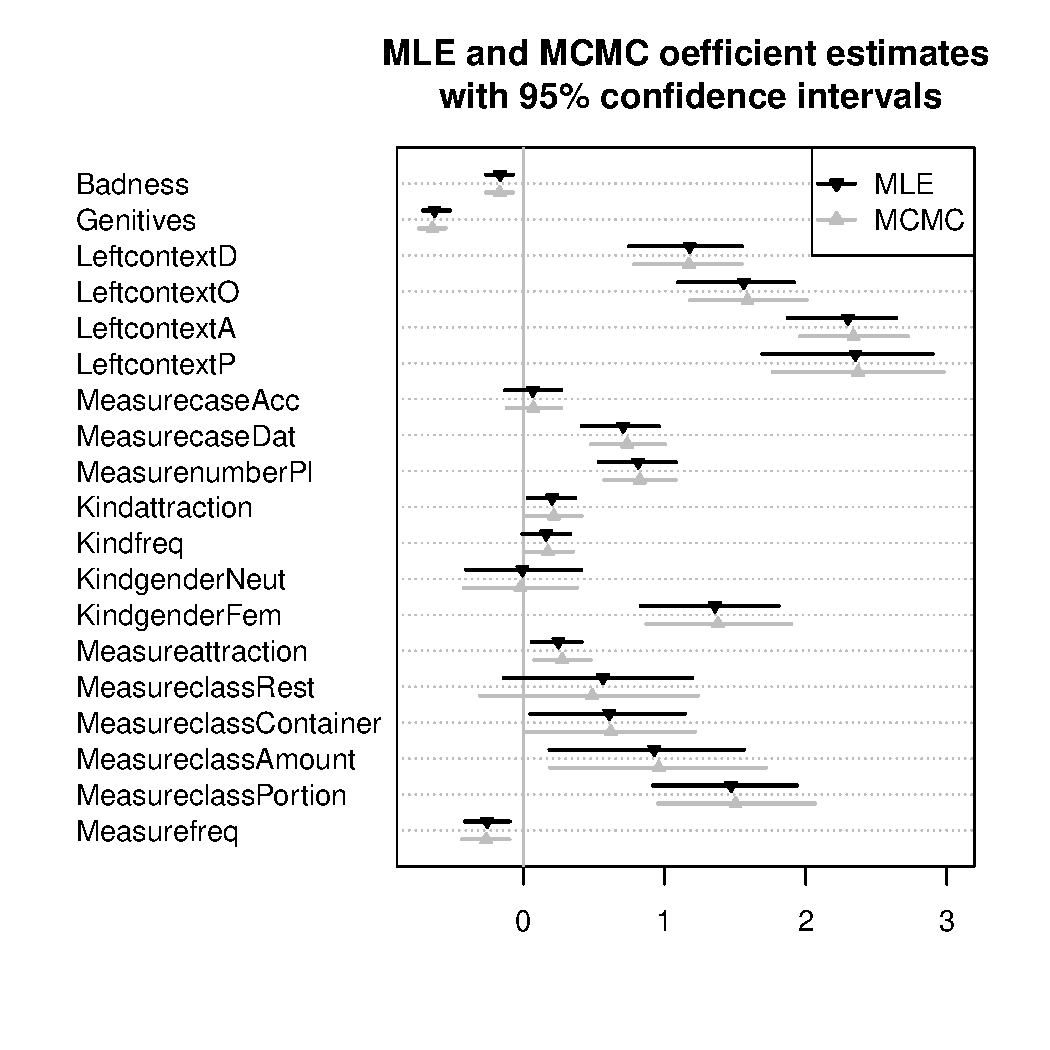
\includegraphics[width=0.85\textwidth]{../R/output/corpus_fixeffs_mle+mcmc}
  \caption{Coefficients (MLE and MCMC) with 95\% confidence intervals (for details see text); the intercept is -4.328 (MLE) and -4.441 (MCMC)}
  \label{fig:fixeffs}
\end{figure}

In this section, I report the results of fitting a multilevel model to the data using R \citep{R}, \textit{lme4} \citep{lme4} for Maximum Likelihood Estimation (MLE) and \textit{rstanarm} \citep{rstanarm} for Bayesian Markov-Chain Monte Carlo (MCMC) estimation (see Section~\ref{sec:rightstatistics}).
The purpose is to model the influence of the regressors specified in Table~\ref{tab:variables} on the probability that the \PGCa\ is chosen over the \NACa.
All regressors from Table~\ref{tab:variables} were included, and the measure lemma and the kind noun lemma were specified as varying-intercept random effects.
The sample size was \textit{n=}5,063 with 1,134 cases of \PGCa\ and 3,929 cases of \NACa.
The results of the estimation are shown in Table~\ref{tab:bigtable} and in Figure~\ref{fig:fixeffs}.
The intercept comprises \textit{Cardinal=Yes}, \textit{Measurecase=Nom}, \textit{Kindgender=Masc}, \textit{Measureclass=Physical}, and 0 for all numeric z-transformed regressors.
It is -4.328 for the ML estimate and -4.441 for the MCMC estimate.

The regressors with the measure lemma as their unit of reference have no within-measure lemma variance, and the \textit{glmer} function automatically estimates them as \textit{group level predictors} (or \textit{second-level effects}), cf.\ \citet[265--269,302--304]{GelmanHill2006}.
The same goes for those listed with the kind lemma as their unit of reference.
Given the coding of the response variable, coefficients leaning to the positive side can be interpreted as favouring the \PGCa.

\begin{sidewaystable}
  \centering
  \resizebox{\textheight}{!}{
  \begin{tabular}{llrlp{0.5em}rrp{0.5em}rrp{0.5em}rrp{0.5em}cc}
      Model & Regressor & \multicolumn{1}{l}{\pPB} & Factor && \multicolumn{2}{l}{Coefficient} && \multicolumn{2}{l}{CI low} && \multicolumn{2}{l}{CI high} && \multicolumn{2}{l}{CI excludes 0} \\
      level &                   &       & level     && \multicolumn{1}{l}{MLE} & \multicolumn{1}{l}{MCMC} && \multicolumn{1}{l}{MLE} & \multicolumn{1}{l}{MCMC} && \multicolumn{1}{l}{MLE} & \multicolumn{1}{l}{MCMC} && \multicolumn{1}{l}{MLE} & \multicolumn{1}{l}{MCMC} \\\midrule
       First     & Badness           &  0.002 &           && -0.152 & -0.155 && -0.247 & -0.247 && -0.061 & -0.065 && * & * \\
                 & Cardinal          &  0.001 & No        &&  1.189 &  1.222 &&  0.862 &  0.927 &&  1.466 &  1.496 && * & * \\
                 & Genitives         &  0.001 &           && -0.693 & -0.711 && -0.768 & -0.801 && -0.592 & -0.616 && * & * \\
                 & Measurecase       &  0.001 & Acc       &&  0.030 &  0.031 && -0.150 & -0.159 &&  0.212 &  0.222 &&   &   \\
                 &                   &        & Dat       &&  0.705 &  0.729 &&  0.455 &  0.465 &&  0.944 &  0.995 && * & * \\[0.5\baselineskip]
       
       Second    & Kindattraction    &  0.020 &           &&  0.225 &  0.244 &&  0.049 &  0.056 &&  0.393 &  0.422 && * & * \\
       (Kind)    & Kindfreq          &  0.095 &           &&  0.146 &  0.164 && -0.023 & -0.016 &&  0.301 &  0.341 &&   &   \\
                 & Kindgender        &  0.001 & Neut      &&  0.021 &  0.013 && -0.367 & -0.409 &&  0.392 &  0.435 &&   &   \\
                 &                   &        & Fem       &&  1.269 &  1.289 &&  0.800 &  0.788 &&  1.709 &  1.783 && * & * \\[0.5\baselineskip]
       
       Second    & Measureattraction &  0.001 &           &&  0.282 &  0.299 &&  0.106 &  0.102 &&  0.447 &  0.515 && * & * \\
       (Measure) & Measureclass      &  0.001 & Container &&  0.252 &  0.257 && -0.265 & -0.303 &&  0.788 &  0.813 &&   &   \\
                 &                   &        & Rest      &&  0.421 &  0.379 && -0.209 & -0.378 &&  1.063 &  1.091 &&   &   \\
                 &                   &        & Amount    &&  0.831 &  0.889 &&  0.215 &  0.220 &&  1.432 &  1.569 && * & * \\
                 &                   &        & Portion   &&  1.217 &  1.253 &&  0.675 &  0.689 &&  1.684 &  1.840 && * & * \\
                 & Measurefreq       &  0.005 &           && -0.231 & -0.232 && -0.363 & -0.395 && -0.079 & -0.073 && * & * \\

  \end{tabular}
  }
  \caption{Coefficient table comparing Maximum Likelihood Estimation (MLE, with 95\% bootstrap confidence interval) and `Bayesian' Markov-Chain Monte Carlo estimation (MCMC); the intercept is -4.328 (MLE) and -4.441 (MCMC)}
  \label{tab:bigtable}
\end{sidewaystable}

Standard diagnostics for MLE show that the model quality is quite good.
Generalised variance inflation factors for the regressors were calculated to check for multicollinearity \citep{FoxMonette1992,ZuurEa2010}, and none of the corrected $\text{GVIF}^{1/2\text{df}}$ was higher than 1.6.
Nakagawa \& Schielzeth's pseudo-coefficient of determination is $R_m^2=0.409$ and $R^2_c=0.495$ (see \citealp{Gries2015} for a basic introduction to these $R^2$ measures, or else \citealp{NakagawaSchielzeth2013}).
The rate of correct predictions is 0.843, which means a proportional reduction of error of $\lambda=0.297$.
The lemma intercepts have standard deviations of $\sigma_{\text{Measurelemma}}=0.448$ and $\sigma_{\text{Kindlemma}}=0.604$.

The coefficient estimates are specified in Table~\ref{tab:bigtable} for each regressor (or regressor level) in the columns labelled \textit{Coefficient}.
For a robust quantification of the precision of the estimation, I ran a parametric bootstrap (using the \mbox{\textit{confint.merMod}} function from \textit{lme4}) with 1,000 replications and using the percentile method for the calculation of the intervals.
The resulting 95\% bootstrap confidence intervals are reported in Table~\ref{tab:bigtable} in the columns labelled \textit{CI low} and \textit{CI high} (= upper and lower 2.5th percentiles).
The column \textit{CI excludes 0} shows an asterisk for those intervals that do not include 0.
Furthermore, for each regressor, a p-value was obtained by dropping the regressor from the full model, re-estimating the nested model, and comparing it to the full model.
Instead of inexact Wald approximations and Likelihood Ratio Tests, I used a drop-in bootstrap replacement for the Likelihood Ratio Test from the function \textit{PBmodcomp} from the \textit{pbkrtest} package \citep{HalekohHojsgaard2014}.
I call the corresponding value $p_{\text{PB}}$, and it is given in the respective columns in Table~\ref{tab:bigtable}.
Only \textit{Kindfreq} ($\mpPB=0.095$) can be seen as slightly too high to be convincing (non-significant).

Finally, I show that MCMC does not necessarily lead to different results.
Actually, given the low complexity of the model and the large sample size, it would be surprising if they did (see Section~\ref{sec:rightstatistics}).
The model was re-estimated using the \textit{stan\_glmer} function from the \textit{rstanarm} package, which provides an \textit{lme4}-compatible syntax for estimating common model types with the \textit{stan} software \citep{CarpenterEa2017}.
The algorithm was run with 4 chains and 1,000 iterations, and I used plausible default priors.
Most notably, priors for coefficients were specified as $\mathcal{N}(0,10)$ because coefficients higher than 10 or lower than $-10$ are extremely rare in well-specified models on appropriate data.%
\footnote{Consider that with a coefficient of 10, each increase by 1 in the regressor variable increases the odds by $exp(10)=22,026.47$.
To reliably estimate such coefficients, extremely large samples would be required.}
The algorithm converged, and for all coefficients, the $\hat{R}$ diagnostic was exactly 1.
The resulting coefficients and intervals as well as an * for ``confidence interval does not contain 0'' are also given in Table~\ref{tab:bigtable} in the columns labelled \textit{MCMC}.
Both methods lead to exactly the same results (minus negligible numerical differences) as expected given the modest complexity of the model structure and the large sample size.
The signs and magnitudes of the coefficients are identical, and the confidence intervals have the same width and symmetry properties.
Figure~\ref{fig:fixeffs} illustrates this by also showing both estimates.
Since both estimators converge, I only interpret the MLE model in the next section.


%%%%%%%%%%%%%%%%%%%%%%%%%%%%%%%%%%%%%%%%%%%%%%%%%%%%%%%%%%%%%%%%%%%%%%%
%%%%%%%%%%%%%%%%%%%%%%%%%%%%%%%%%%%%%%%%%%%%%%%%%%%%%%%%%%%%%%%%%%%%%%%


\subsection{Interpretation}
\label{sec:interpretation}

% ATTRACTION

\begin{figure}[h!]
  \centering
  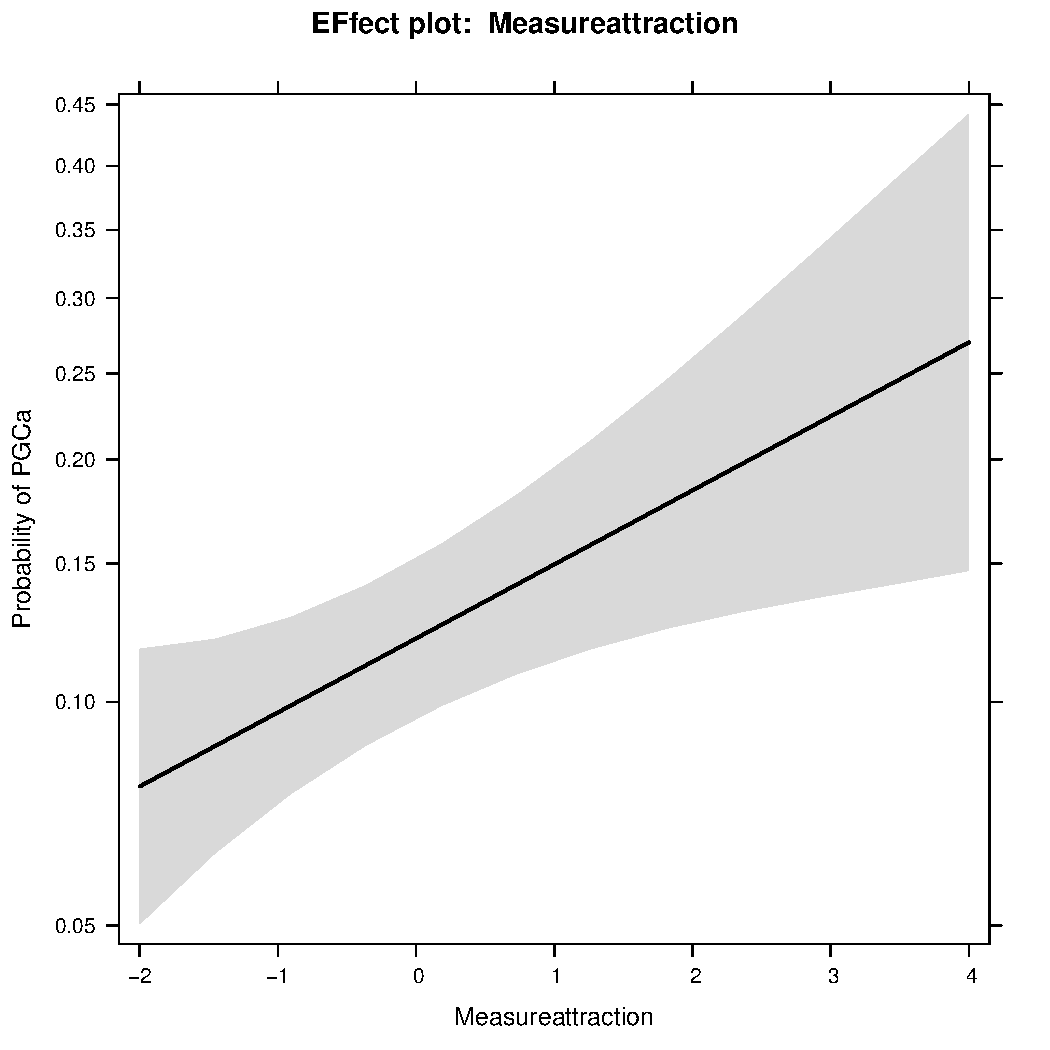
\includegraphics[width=0.5\textwidth]{../R/output/corpus_Measureattraction}~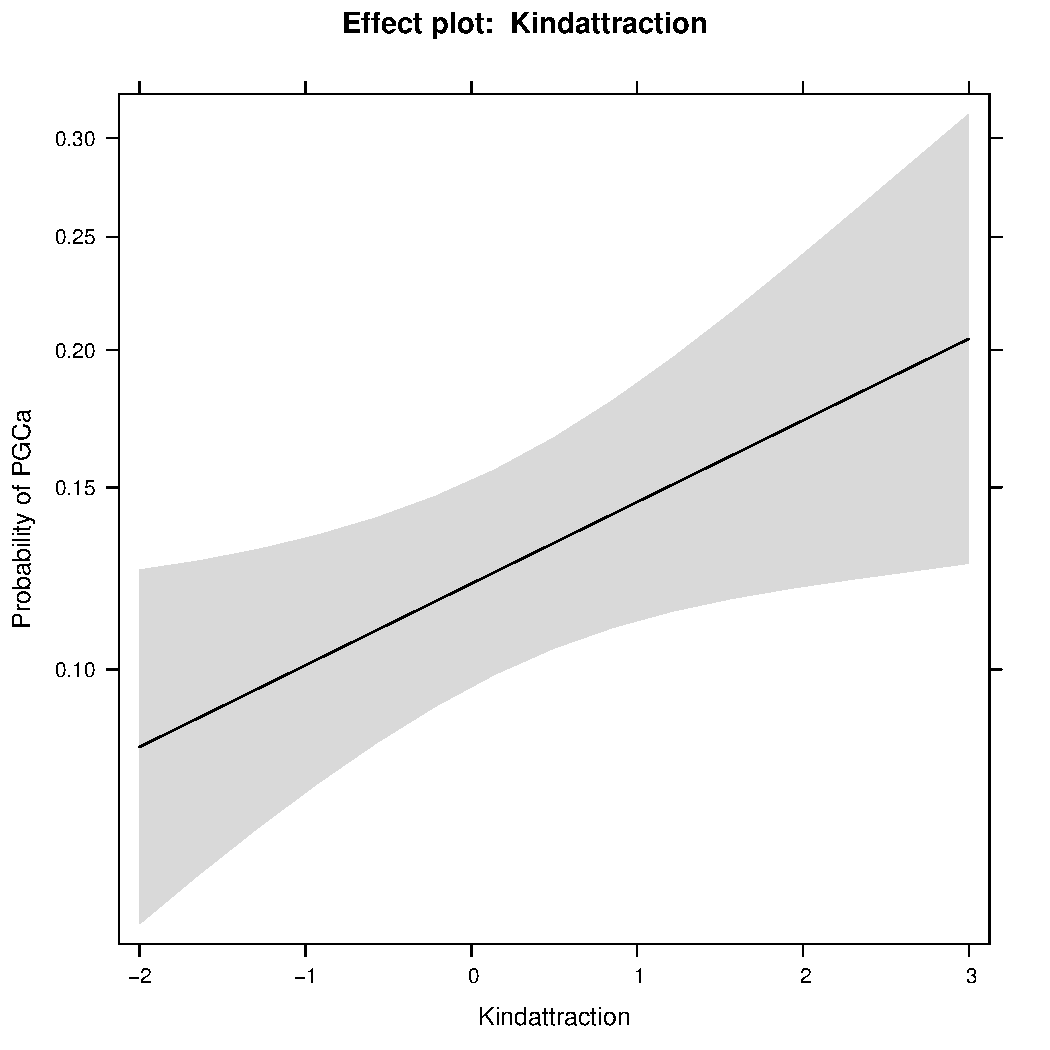
\includegraphics[width=0.5\textwidth]{../R/output/corpus_Kindattraction}
  \caption{Effect plots for the regressors \textit{Measureattraction} and \textit{Kindattraction}; y-axes are not aligned}
  \label{fig:eff:attraction}
\end{figure}

The results reported in Section~\ref{sec:corpushierarchicalmodel} generally confirm the hypotheses from Section~\ref{sec:analyses}.
First, the prototypicality effect related to the non-alternating \PGCd\ and \NACb\ can be shown (see the effect plots in Figure~\ref{fig:eff:attraction}).%
\footnote{Effect plots were created using the \textit{effects} package \citep{Fox2003}.
They show the changes in probability for the outcome (y-axis) dependent on values of a regressor (x-axis) at typical values of all other regressors.
The vertical bars (categorical variables), and the grey areas (continuous variables) are asymptotic 95\% confidence intervals calculated from \textit{glmer}.
They are not bootstrapped.
Readers should be aware that the axes are specifically scaled so as to result in a linear plot, and that the range of the axes varies between plots.}
The effect is as expected:
if a lemma appears relatively more often in the \PGCd\ (compared to its frequency in the \NACb), the \PGCa\ tends to be chosen over the \NACa\ with this specific lemma.
The effect for measure nouns is stronger, and it was estimated with higher precision.

An interesting picture emerges for the lemma frequencies.
A higher-than-average lemma frequency of measure nouns favours the \NACa\ ($\beta_{\text{Measurefreq}}=-0.231$, $\mpPB=0.005$), which is as expected if we assume at least a tendency for highly grammaticalised items to be more frequent.
With kind nouns, higher frequency seems to favour the \PGCa ($\beta_{\text{Kindfreq}}=0.146$, $\mpPB=0.095$).
However, there is no clear theoretical interpretation (see Section~\ref{sec:analyses}), and the estimate is imprecise (not significant at $\alpha=0.05$, see above).
The effect can therefore be ignored or treated as a nuisance variable.


% GRAMMATICALISATION
% => lemmas and lemma classes

\begin{figure}[h!]
  \centering
  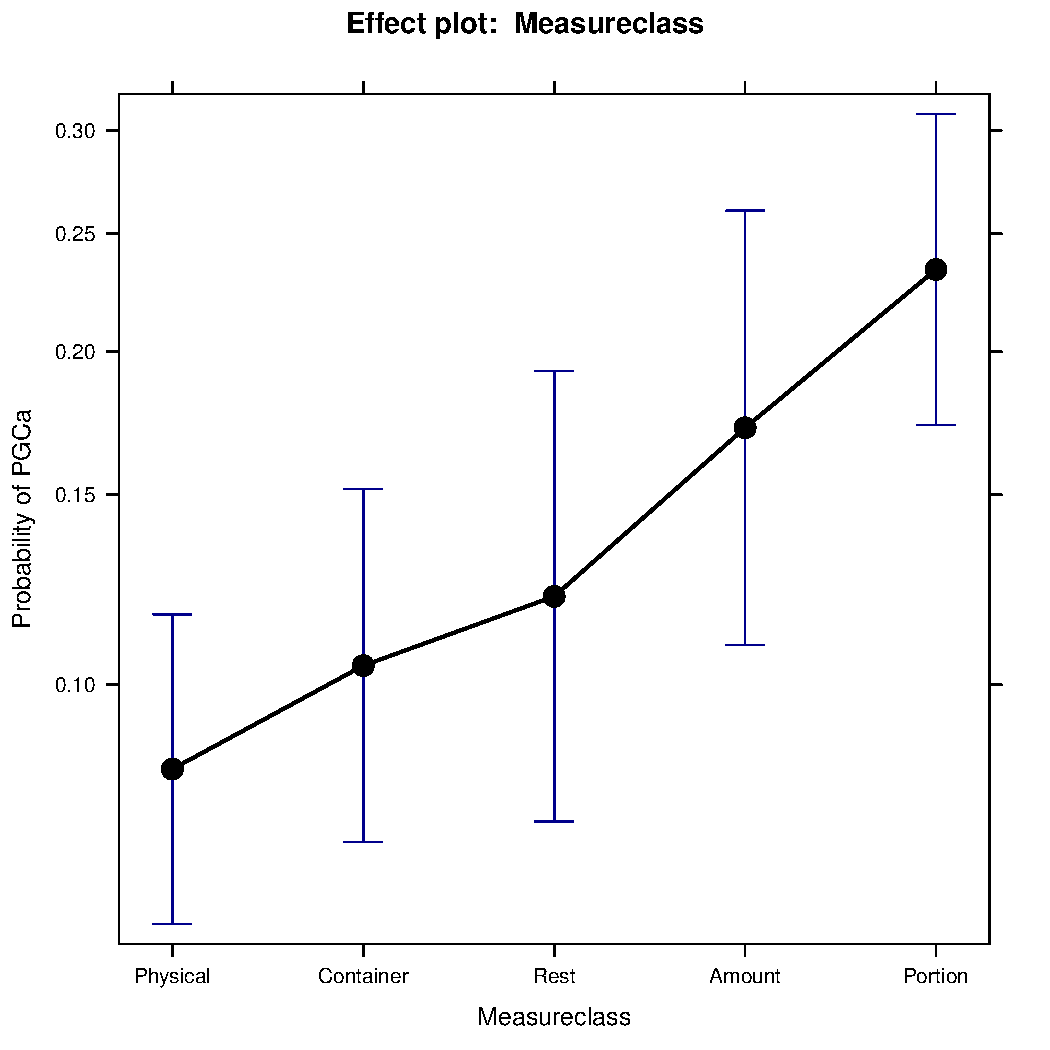
\includegraphics[width=0.5\textwidth]{../R/output/corpus_Measureclass}
  \caption{Effect plot for the regressor \textit{Measureclass}}
  \label{fig:eff:measureattraction}
\end{figure}

In Section~\ref{sec:analyses}, it was also hypothesised that classes of measure nouns with a higher degree of grammaticalisation should favour the \NACa.
The \textit{Measureclass} second-level predictor was successfully estimated ($\mpPB=0.001$).
Looking at the effect plot in Figure~\ref{fig:eff:measureattraction}, it is evident that abstract non-referential physical measure nouns (such as \textit{Gramm} `gram' or \textit{Liter} `litre') with a high degree of grammaticalisation favour the \NACa.
At the other end of the scale, nouns denoting natural portions like \textit{Haufen} `heap', \textit{Bündel} `bundle', \textit{Schluck} `gulp' favour the \PGCa.
These are referential nouns, confirming the hypothesis that it is prototypical of the PGC to contain two referential nouns, while the NAC prototypically only contains one (the kind noun).

% CARDINALS

\begin{figure}[h!]
  \centering
  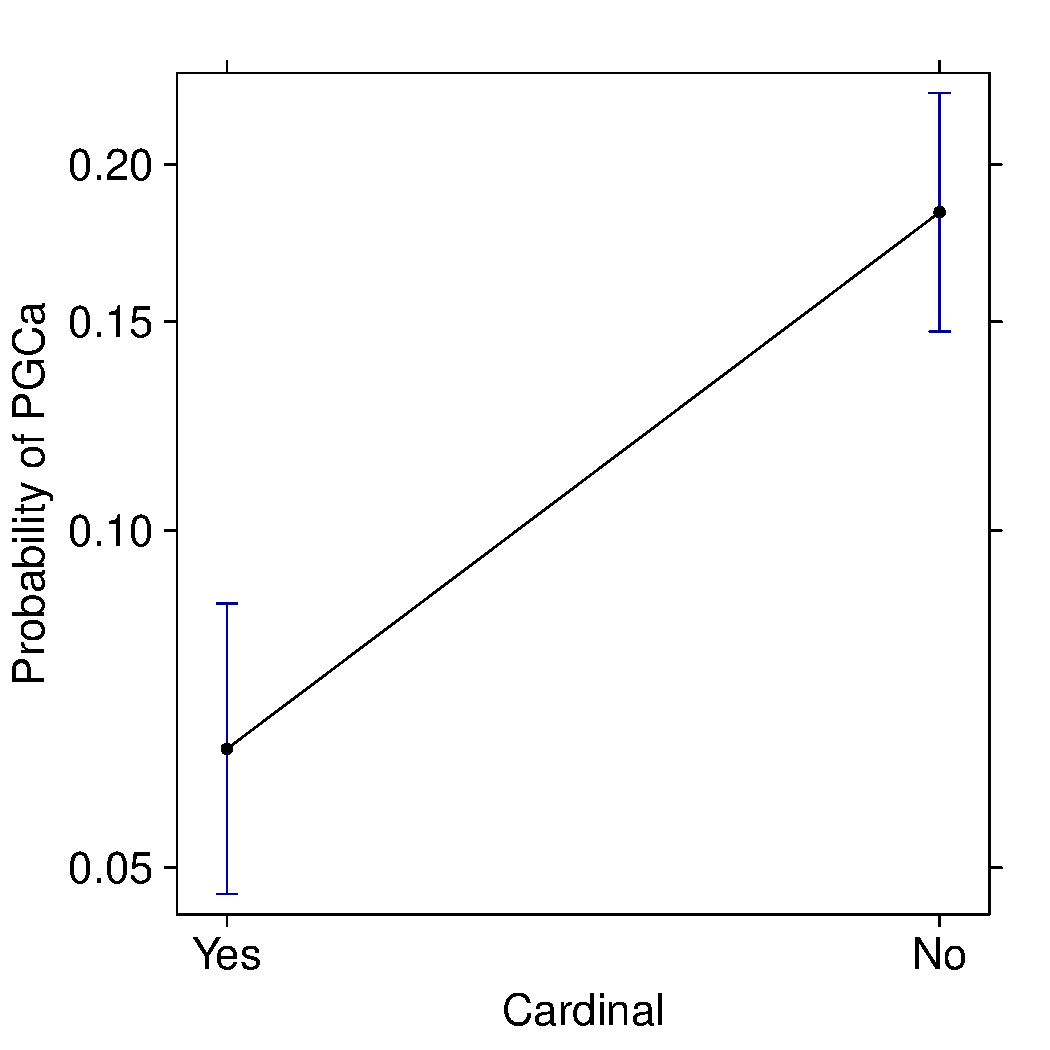
\includegraphics[width=0.5\textwidth]{../R/output/corpus_Cardinal}
  \caption{Effect plot for the regressor \textit{Cardinal}}
  \label{fig:eff:leftcontext}
\end{figure}

I now turn to the predicted effect of cardinals as modifiers of the measure noun.
Figure~\ref{fig:eff:leftcontext} shows that cardinals indeed influence the choice of the alternant ($\mpPB=0.001$), and that cardinals have a strong tendency to co-occur with the \NACa.
This effect was predicted in Section~\ref{sec:analyses}.

% REGISTER
% => Badness
% => Genitives

The style-related proxy variables point to the expected direction.
Increased \textit{Badness} of the document favours the \NACa\ ($\beta_{\text{Badness}}=-0.152$, $\mpPB=0.002$), and so does a lower density of genitives ($\beta=-0.693$, $\mpPB=0.001$).
While these are merely proxies to style (and partially circular in the case of \textit{Genitives}), this result can at least encourage future work into stylistic effects. 

% NUISANCE
% => dative effect
% => frequency

The influence of \textit{Measurecase} ($\mpPB=0.001$) is as predicted in previous analyses (see Section~\ref{sec:analyses}).
A measure noun in the dative favours the \PGCa\ with $\beta_{\text{MeasurecaseDat}}=0.705$ (compared to the nominative, which is on the intercept).
Although \textit{Measurecase} is a nuisance variable in the context of this study, convergence with previous work strengthens its validity.

%%%%%%%%%%%%%%%%%%%%%%%%%%%%%%%%%%%%%%%%%%%%%%%%%%%%%%%%%%%%%%%%%%%%%%%
%%%%%%%%%%%%%%%%%%%%%%%%%%%%%%%%%%%%%%%%%%%%%%%%%%%%%%%%%%%%%%%%%%%%%%%
%%%%%%%%%%%%%%%%%%%%%%%%%%%%%%%%%%%%%%%%%%%%%%%%%%%%%%%%%%%%%%%%%%%%%%%


